%===================================== CHAP 1 =================================
\chapter{Introduction}

This chapter will introduce the thesis by providing a background for the problem and research area. It will also explain the motivation behind the thesis, and what we aspire to contribute to the field, before composing this into a set of goals and research questions. Finally, the chapter will describe the research method and the structure of the thesis.

\section{Background}

\textit{Introduce the thesis and describe how it is a continuation of the specialization project. Both the web interface as well as the case study in facial recognition with expressions.}

\begin{itemize}
    \item Maybe start with an overall general introduction to the problem, i.e. that it is in the field of artificial neural networks and how they behave, specifically images. Ex. this thesis deals with the field of ...
\end{itemize}

The thesis is concerned with artificial neural networks and the use of visualization techniques to gain an understanding of their behaviour. Furthermore, the thesis explores a novel approach to improve the accuracy of facial recognition networks. The work presented in the thesis is a continuation from the results of the Specialization Project. 

\noindent The problem to be solved in this thesis can be divided into two parts:
\begin{enumerate}
    \item A visualization tool for deep learning
    \item A case study in facial recognition
\end{enumerate}

\noindent The first part proposes a tool for visualizing data produced during the training of an artificial neural network. This visualization tool should be implemented in the form of a web interface where users can upload and run their Python scripts for creating and training such networks. The tool should use established visualization techniques to generate visualizations for the user in order to help them gain insight into why their networks behave as they do and, by extension, how they can be improved. \\

\noindent A prototype of this interface has been implemented as part of the Specialization Project and will act as a basis as we continue the development. A more thorough description of the prototype, as well as an overview of what to implement for this thesis, will be presented in chapter 4. \\

\noindent The purpose of the case study in the second part will be to explore whether it is possible to exploit facial expression data in order to improve an artificial neural network for face recognition. We theorize that a network with access to facial expression data could learn the alterations of features associated with various expressions, and apply this to recognize faces which differ in the corresponding features. \\

\noindent The case study in the second part will act as an example of how to utilize the implemented visualization tool when working with artificial neural networks. In this part, the purpose will be to explore whether it is possible to exploit facial expression data in order to improve an artificial neural network for face recognition. We theorize that a network with access to facial expression data could learn the alterations of features associated with various expressions, and apply this to recognize faces which differ in the corresponding features. We intend to create three different networks, where one is using a standard implementation and functions as a benchmark for the other two, which will be experimental.


\section{Motivation}

\noindent In the modern computer science landscape, artificial neural networks are on the rise. They have enjoyed considerable success in a plethora of fields and there exist a multitude of frameworks dedicated to creating and training such networks. Among the frameworks are TensorFlow and Caffe2, which are open-source projects backed by tech giants Google and Facebook, respectively. However, an issue with artificial neural networks is that they have been notoriously difficult to understand. Being dissatisfied with this knowledge vacuum, researchers have developed a number of visualization techniques to help gain insight into the inner workings of a network. Unfortunately, unlike the building of networks, there does not exist an extensive amount of options when it comes to facilitating the creation of visualizations. To combat this shortage, we aim to design and develop a tool that provides users with easy access to visualization techniques through a convenient user interface. More specifically, we plan to fill the void of an advanced visualization tool for the machine learning frameworks Theano and TensorFlow through the use of Keras, a high-level API supporting both frameworks. The tool would aid researchers using these popular frameworks to gain a better understanding of their networks and how to improve them, thus enabling further research. \\

\noindent One of the fields where artificial neural networks have been successfully applied is the area of face recognition. In addition to developing the visualization tool, we also propose a case study in the face recognition field, where we intend to investigate a theory regarding facial recognition neural networks. We postulate that an approach that utilizes the information available in facial expressions may experience greater accuracy than one that tries to overcome expressions through invariance. The hypothesis will be examined by adapting a well known artificial neural network architecture to the face recognition domain to create two networks: one conventional to act a basis to be evaluated against and one experimental that exploits facial expression data. \\

\section{Contributions}

The thesis introduces a visualization tool, implemented as a web interface, that can help researchers and engineers gain a better understanding of the behaviour of their artificial neural networks and how to improve them. The effort will be concentrated on generating visualizations for networks whose input data reside in the 2D-image domain. The tool should be easily extensible, in regard to adding new visualization techniques and customizing the tool to a different machine learning framework. \\

\noindent The thesis also explores the face recognition field by investigating if the exploitation of facial expression data in face recognition systems could be beneficial.

\section{Research Questions}

\textbf{RQ1:} How can we develop a tool to improve the understanding of the behaviour of an artificial neural network? \\
\textbf{RQ2:} How can facial expression data be utilized to improve a face recognition system?

\section{Research Methodology}

This section will explain the research method used in our thesis. Note that this is not to be confused with the more specific system development method, which is the explanation and documentation of how the suggested systems are implemented. This will be further addressed in chapter 4. The research methodology is the combination of research strategies and data generation methods to be used in the thesis. Even though our research consists of two separate problems, we plan to address them simultaneously, and will employ similar methods for both. Thus, parts of this section discusses the research in general instead of separately for each research question.

\subsection{Research Strategy}

Oates proposed six different strategies for answering research questions. Since both of our questions are concerned with the implementation of some kind of computer system, it is natural to employ the design and creation strategy, which focuses on developing new information technology (IT) products, or so called artefacts. March \& Smith defines four types of IT artefacts: constructs, models, methods and instantiations. Instantiations are working systems that demonstrates that constructs, models, methods, ideas or theories can be implemented in a computer-based system. The research output in our case will be two instantiations: the implemented visualization tool, and an implementation of a face recognition system incorporating a novel idea. \\

\noindent Vaishnavi \& Kuechler present an iterative process typical for design and creation illustrated in \textbf{Fig. \ref{dsr-cycle}}. The process suggests a "learning through making" approach and involves five steps, followed in an iterative cycle: awareness of problem, suggestion, development, evaluation and conclusion. The first step is to study existing literature and research to uncover the need for something. The second step provides a creative leap from the need to a simple idea of a solution. Then, the idea is implemented in the third step, followed by an evaluation of this implementation and an explanation of possible deviations from the expectation in the fourth step. Finally, in the fifth step, the result is documented, and the knowledge gained as well as any possible future work is identified. \\

\begin{figure}[h!]
    \centering
        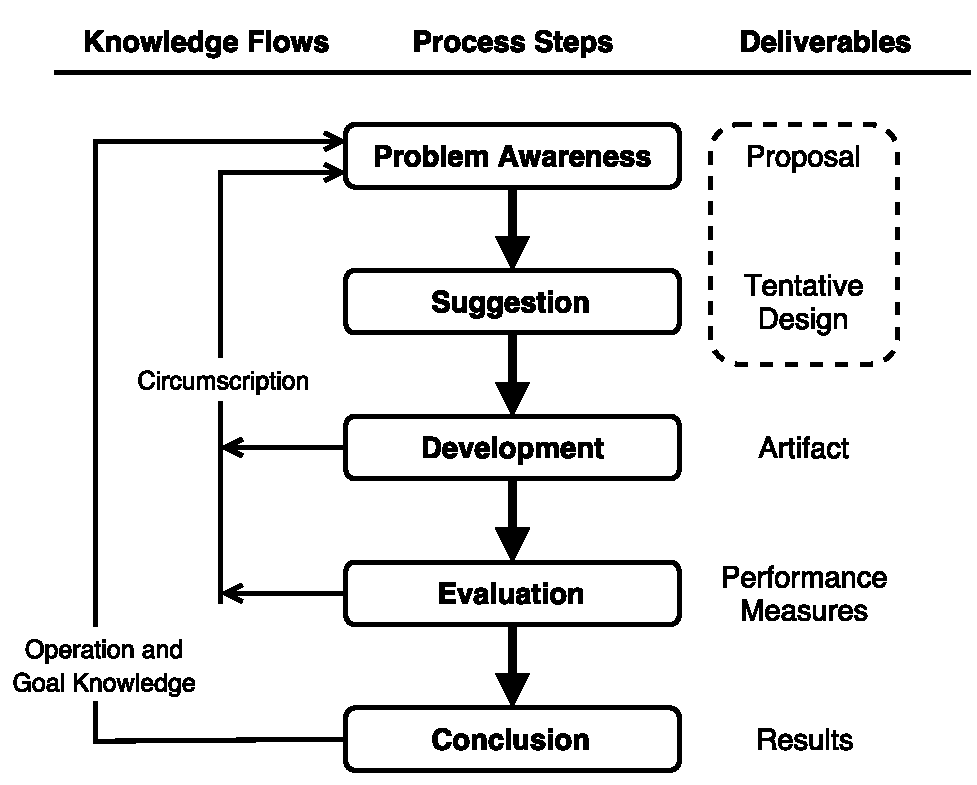
\includegraphics[width=0.7\textwidth]{fig/dsr-cycle.pdf}
        \caption{Design Science Research Process Model (DSR Cycle)}
        \label{dsr-cycle}
\end{figure}

\noindent For the visualization tool, the first couple of iterations of this cycle has already been conducted in the Specialization Project. The result of this project included many pointers on future work, that will be addressed in this thesis. We will continue to repeat the process until we can conclude with an implementation that is satisfactory according to our research goals and questions. For the case study, however, no development was conducted in the Specialization Project. The focus was rather on the first two steps, namely to define the problem and suggest a solution. In this thesis, we will continue the process by implementing the suggested solution, and continue to evaluate and improve it until we reach a conclusion.\\

\subsection{Data Generation Methods}

The data that will be used in this thesis will mainly be qualitative data in the form of documents. For the implementation of the visualization tool, articles on various visualization techniques that can aid in understanding artificial neural networks will be essential. We will also make use of documentation of the frameworks and technologies used in implementation. To document the implemented tool and capture our research strategy, we will generate our own documents using architectural diagrams and user manuals. \\

\noindent For the case study, we will need a large amount of images. Since our case study is concerned with the field of face recognition with expressions, we require images of people with different facial expressions, photographed under various conditions, labeled with identification and expression. There exist several datasets created solely for the purpose of face recognition, but the challenge will be to find one of appropriate size, with the right amount of metadata. The larger datasets examined have a tendency to be expensive or lack availability. The chosen dataset will be used to both train the networks and validate their performance afterwards.

\subsection{Data Analysis}

To present the results of the visualization tool, we will make use of well known artificial neural networks, and show the visualizations produced at various stages of training. Since the results are images, we will need to perform quantitative data analysis on these images. The goal will be to identify connections between the visualizations and the behaviour of the networks, both in terms of why they may perform well and why they may struggle. \\

\noindent Qualitative data analysis will be performed on the results of the case study. The prediction accuracy of an artificial neural network is defined as the percent of correctly classified inputs, in our case images. The accuracy of our implemented network incorporating the proposed will be measured against the accuracy of the baseline network. By comparing these, we should be able to determine whether exploiting expressions in such a way could be beneficial.


\begin{itemize}
    \item \textbf{Awareness of problem:} The awareness of a problem may come from studying existing literature and research, and discovering a need for something.
    \item \textbf{Suggestion:} A creative step for developing a simple idea of how the problem could be solved.
    \item \textbf{Development:} The implementation of the idea in the previous step.
    \item \textbf{Evaluation:} Evaluating the implementation and explain possible deviations from the expectation.
    \item \textbf{Conclusion:} The result is documented. Knowledge gained and any possible future work is identified.
\end{itemize}

\begin{itemize}
    \item \textbf{Constructs:} Concepts or vocabulary used in a particular IT-related domain.
    \item \textbf{Models:} Combination of constructs that represent a situation and are used to aid problem understanding and solution development.
    \item \textbf{Methods:} Guidance on the models to be produced and process stages to be followed to solve problems using using IT.
    \item \textbf{Instantiations:} Working system that demonstrates that constructs, models, methods, ideas, genres or theories can be implemented in a computer-based system.
\end{itemize}


\noindent To achieve the goals of our thesis, we will follow this process. First, we identify the gap by examining related work and proposing our own solution. The development follows as we implement the proposed solution. We evaluate the implementation, and if there are any deviations keeping the result from being satisfying, we repeat the cycle. Finally, the result should be satisfactory, and we can document the finished implemented solution.



\section{Thesis Structure}

\begin{table}[!h]
\begin{center}
\begin{tabular}{ | l | p{8cm} |}
\hline
\textbf{Chapter/Appendix} & \textbf{Description} \\ \hline
1. Introduction & Provides an overview of the project and the thesis. \\ \hline
2. Background Theory & Provides the theory relevant for the project. \\ \hline
3. Related Work & ... \\ \hline
4. Implementation & Describes the web interface in terms of architecture and technologies used. \\ \hline
5. Results & Presents the results from the case study. \\ \hline
6. Discussion & Discussion of the results from the case study as well as the use of the web interface. \\ \hline
7. Conclusion & Provides a short conclusion and some pointers on future work. \\ \hline
8. Future Work & ... \\ \hline
A. Installation & A step by step wizard for how to install and setup the interface. \\ \hline
B. User Manual & How to use the web interface. \\ \hline
C. API & Provides an overview of the API and explanation of the callbacks available. \\ \hline
\end{tabular}
\end{center}
\caption{Overview of the thesis structure}
\label{tab:1}
\end{table}

\cleardoublepage